\question 若8个字(字长32位)组成的位示图管理内存,假定用户归还一个块号为100的内存块时,它对应位示图的位置为(
~)。假定字号、位号、块号均从1开始算起,而不是从0开始
\par\fourch{字号为3,位号为5}{\textcolor{red}{字号为4,位号为4}}{字号为3,位号为4}{字号为4,位号为5}
\begin{solution}本题考查位示图的字号和位号计算,考生一看到就应该想到要用画草图的方法解答。
解法一:由位示图的盘块号到字号、位号的转换公式得:
若回收的盘块号为b,则字号i=(b-1)/(n+1),位号j=(b-1)\%n+1;
现在b=100,n=32,所以i=(100-1)/(32+1)=3,j=(100-1)\%32+1=4;
所以字号为4,位号为4,答案选B。
解法二:根据题意,画出位示图的草图如图4-11所示。
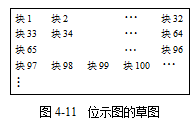
\includegraphics[width=2.02083in,height=1.32292in]{computerassets/4905E5C3F3E6FE52866D6CF2A0B188A5.png}

通过图4-11,发现100块在第4行第4列,所以字号为4,位号为4。答案选B。
这类题如果是选择、填空等非主观题,那么推荐用解法二(画图法)解决。
\end{solution}
